\documentclass[a4paper,10pt,twocolumn,uplatex]{jsarticle}
\usepackage{style/nislab,style/resume}

%---------------------------------------------------------------------
% レジュメ種別・日付設定(要変更)
% \type{} 1:修士論文諮問会 2:卒業論文発表会 3:月例発表会 4:研究室合同発表会
%---------------------------------------------------------------------
\type{3}
\year{2023}
\month{1}
\date{14}

%---------------------------------------------------------------------
% ページ番号設定(要変更)
%---------------------------------------------------------------------
\setcounter{page}{7}

%---------------------------------------------------------------------
% 変更不要
%---------------------------------------------------------------------
\begin{document}

%---------------------------------------------------------------------
% タイトル作成部分(要変更)
% \maketitle{タイトル}{title}{名前}{name}
%---------------------------------------------------------------------
\maketitle{未知領域探査のための複数ドローンを利用した \\動的な三次元環境地図生成によるAR 可視化}
{Multiple Drones-Based AR Visualization \\with Dynamic Environmental Maps for Unknown Area Exploration}
{竹内 一真}
{Kazuma Takeuchi}

% --------------------------- Section1  ---------------------------

\section{はじめに}
近年,ドローン用途は急速に成長しており,中でも小型ドローンの特徴である機体の大きさを活かして,人間が入れないような狭い空間での活躍の場も増加しており,将来的には狭小空間の未知領域探査への応用が期待されている\cite{Nonami}.
% しかし,小型ドローンはセンサ搭載制限があるため,障害物回避の支援がないことが多く,衝突の危険性があり,
% また,障害物回避の機能を搭載していても,狭小空間では障害物回避が行えない場面が多く存在する\cite{syohou}.
% そのため,ドローン搭載のカメラ映像を頼りにした手動による操縦を必要とする.
しかし,狭小空間でのドローン飛行は遮蔽物が多く,操縦者は遮られた視点からの操縦を必要とするため,死角領域内のドローン操縦では,ドローンを視認できない中,衝突することなく,安全に操縦する技術が求められる.
% オンボードカメラ搭載ドローンを使用する場合では,操縦者は,ドローンから送られる空撮した映像を元に操縦が可能となる.
% しかし,カメラが前方しか写さないことにより,前方以外の死角が多くなり,状況認識が不十分となるため\cite{Green},狭小空間のように狭く,障害物が多いような環境では,操縦は困難である.

\par
そこで,事前に走行環境をマッピングし作成した三次元環境地図をAugmented Reality(AR)により表示し,死角領域内を可視化することにより,狭小空間での未知領域探査におけるドローン操縦性向上や安全性向上が期待されている\cite{Erat}.
% 事前に走行環境をマッピングすることで三次元環境地図を取得し,空間認識を提供している.
% しかし,狭小空間のドローン操縦において,事前に三次元環境地図を用意することは困難なため,
% 実際の未知領域探査において,ドローンが一からマッピング,自己位置推定などを行う環境でも同じ効果を発揮できるのか示されていない.
% また,ドローンはバッテリー上限が短く,短時間での効率的な探査を必要とする中で\cite{Gupta},一台のドローンのみで探査を行うには多くの時間を要すため,複数ドローンの利用が検討されている.
% 関連研究では一台のドローンのみを想定していたが,複数ドローンを適応する場合,各ドローンのセンサ情報を共有できるシステムが必要である.
しかし,未知領域でのドローン操縦において,事前に三次元環境地図を用意することは困難なため,
ドローンが一からマッピング,自己位置推定などを行う環境でも同じ効果を発揮できるのか示されていない.
また,ドローンはバッテリー上限が短く,短時間での効率的な探査を必要とするため\cite{Gupta},複数ドローンの利用を検討されているが,
環境中のドローンの数が多ければ多いほど,衝突のリスクは高くなり,また,探査領域の重複も考えられる.
% その上,自身が操縦するドローン以外の飛行しているドローンが,これからどこを探査しようとしているのか,どこまで探査したのかを把握できないため,探査範囲の重複を引き起こすことが想定される.
% そのため,各ドローンの位置情報や探査領域を把握できないことによる,複数ドローン間の衝突危険性や探査済み領域の再探査を低減させる,各ドローンのセンサ情報を共有できる操縦方式が必要である.

% しかし,各ドローンの位置情報や探査領域を把握できないことによる衝突危険性や探査済み領域の再探査の非効率性が考えられるため,各ドローンのセンサ情報を共有できるシステムが必要である.
% 本研究では,狭小空間における死角領域内おいて,複数ドローンによる衝突危険性の軽減,効率的な未知領域探査を実現するため,各ドローンのセンサ情報を統合した上で,ARにより操縦者の死角領域内を可視化するシステムを開発する.
本研究では,狭小空間による死角領域内において,未知領域探査へ投入するドローン数の増加に伴う,探査効率の問題を軽減するため,
各ドローンがSLAM(Simultaneous Localization and Mapping)を用いて取得したセンサ情報を統合した上で,ARにより操縦者の死角領域内を可視化する方式を提案する.
% これにより,複数人が協調的にドローンの連携を図り,衝突危険性の低減させた上で,探査効率を向上させる方式を実現し,その有効性を評価する.

% --------------------------- Section2  ---------------------------

\section{提案方式}
% \subsection{概要}
% 本研究では,狭小空間により,操縦者と小型ドローン(以下,ドローン)の間に遮蔽物があり,ドローンを視認できない環境を「死角領域」とする.
% 提案システムを図\ref{fig:outline}に示しており,各ドローンがリアルタイムで走行環境をマッピングし生成された三次元環境地図
% を,ARにより重畳表示することで,死角領域内の空間認識を提供している.
% \par

\begin{figure}[!tb]
  \centering
  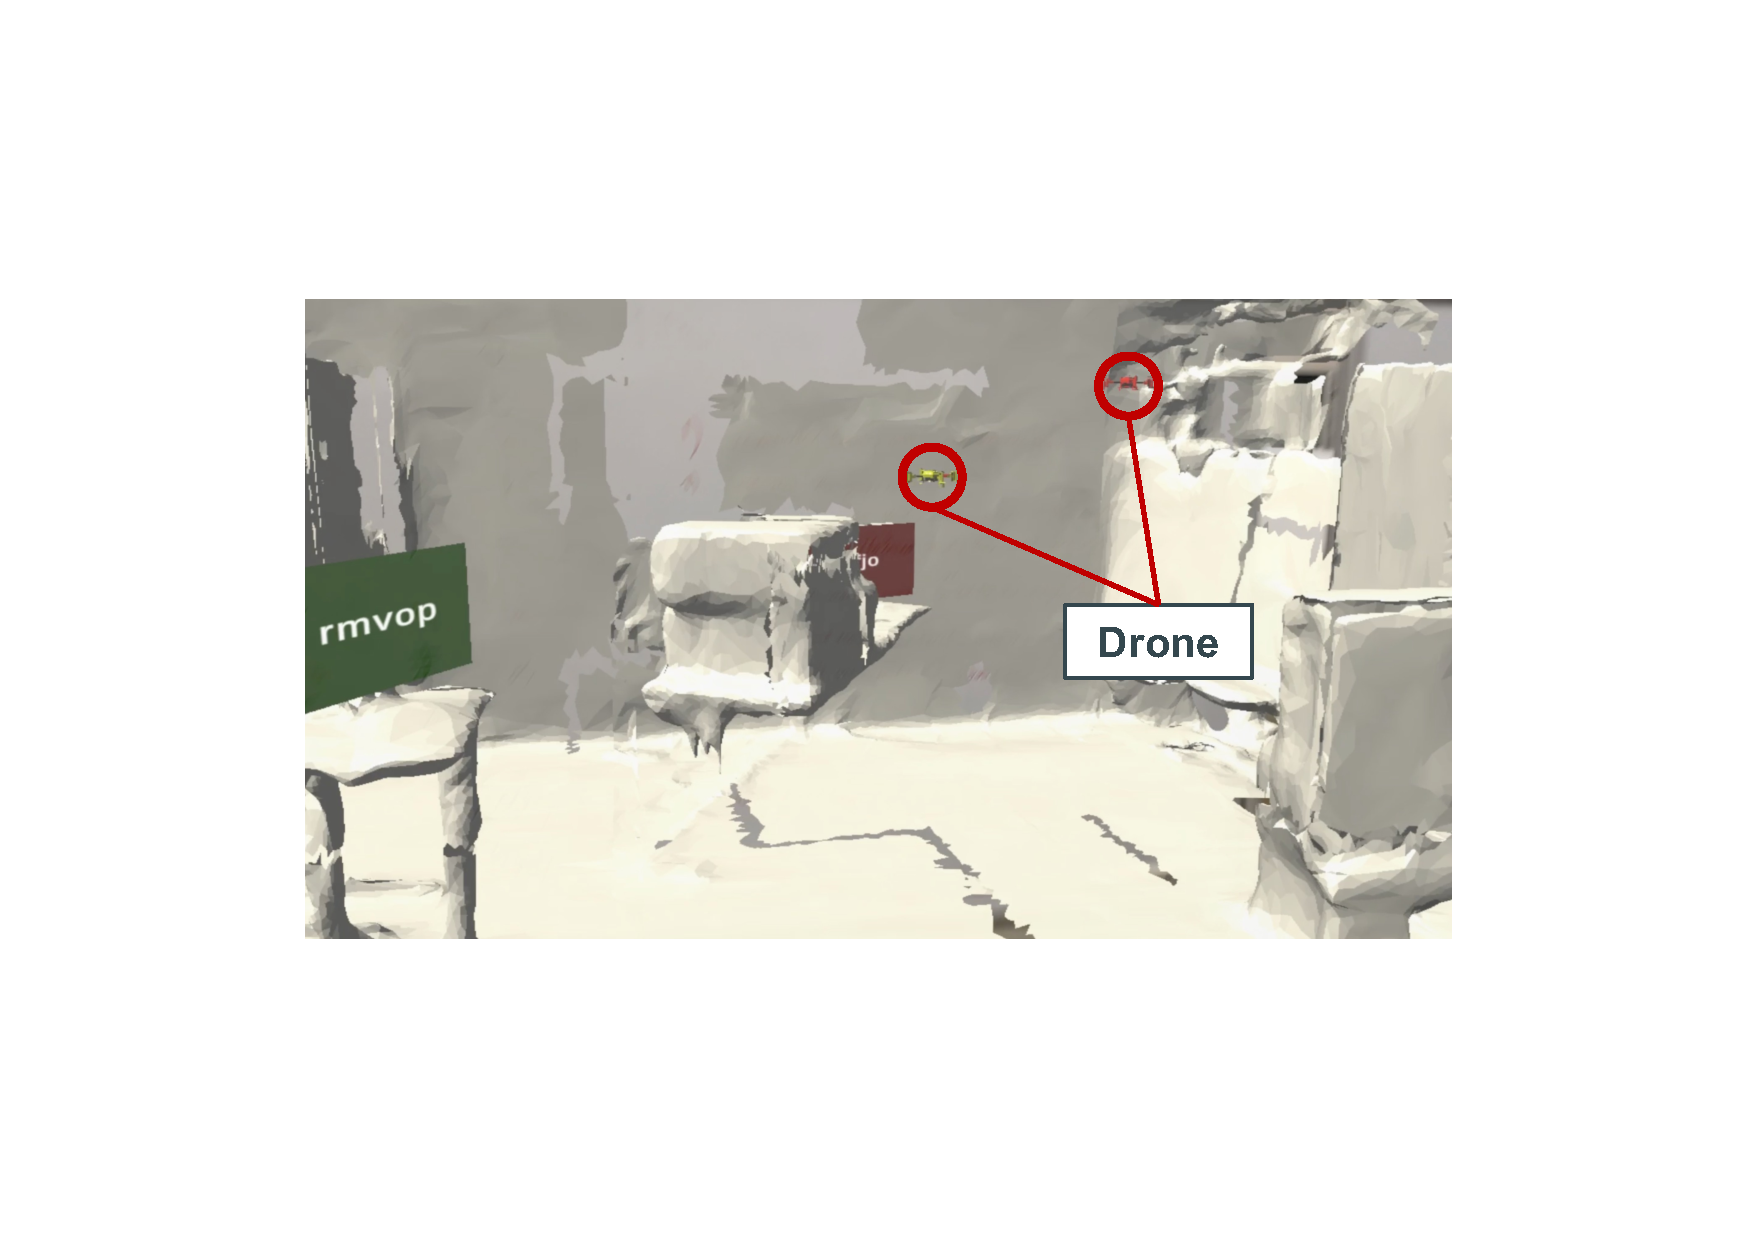
\includegraphics[width=0.9\linewidth]{img/03_propose.pdf}
  \caption{複数ドローン混在時における死角領域内の可視化}
  \label{fig:outline}
\end{figure}


\subsection{死角領域内のAR可視化}
提案方式の概要を\figref{fig:outline}に示す.
先に述べた関連研究\cite{Erat}を元に,操縦者に死角領域内の空間認識を提供する.
ドローンと操縦者の間に遮蔽物が存在する場合,ドローンが飛行している場所が操縦者にとっての死角領域となる.
死角領域が存在すると判断したとき,マッピングした三次元環境地図における遮蔽物を透過した上で,現実環境に重畳表示することで,仮想的に死角領域の空間認識を提供する.
% 操縦者は,死角領域内を飛行するドローンを視認することはできないが,ARによって仮想のドローンと,ドローン周辺の三次元環境を視認することができる.

\subsection{複数ドローンのセンサ情報統合}
本研究におけるドローン操縦では,リアルタイムでマッピングを行い,三次元環境地図を作成する必要がある.
そこで,各ドローンはvSLAM(visual SLAM)であるORB-SLAM2を用いて,単眼カメラで取得した画像から特徴点を抽出し,自己位置推定を行い,
周囲の環境の点群情報を取得する.
しかし,各ドローンの位置情報,生成した点群情報は個々で独立している.
そこで,各ドローンをワールド座標系で管理し,各ドローンの位置情報,点群情報を統合し,操縦者へ提供する仮想的な三次元環境地図,ドローンを生成する.
% また,三次元環境地図はセンサーデータの重ね合わせによって生成しており,膨大な数の点の集合であり,
% データ量が非常に大きいため,点群情報をダウンサンプリングすることでデータ量を削減している.
\subsection{遮蔽物との距離を考慮した危険度の付与}
生成した三次元環境地図を操縦者へ提供し,三次元環境地図上の遮蔽物を透過することで死角領域内を可視化する.
しかし,複数の遮蔽物が存在し,同じ透過度の遮蔽物が重なる場合,どの遮蔽物がドローンに最も近傍であるか認識できなくなり,操縦性の低減や遮蔽物・障害物への衝突危険性を向上させてしまうことが推測できる.
そのため,ドローンから距離の遠い遮蔽物の透明度を向上し,ドローンから距離の近い遮蔽物の透明度を低下させ,その上,ドローンから遮蔽物までの距離に応じて,障害物の色を分類し,近傍の障害物の危険性を警告する機能を開発する.
% することにより,ドローン周辺の遮蔽物を強調表示し,操縦者目線では認識が困難な遮蔽物の形状を把握できる機能を開発する.
% 複数ドローンのセンサ情報を統合することにより,各ドローンの位置情報,点群データ,また画像処理をうまく行えているかの判定を操縦者の装着しているARHMDに送信している.
% 一方で,ARHMDでは仮想表示しているドローンが近傍の障害物へ衝突しそうな場合に,衝突判定のデータをサーバへ送信している.
% これにより,操縦者にとっての死角領域内がどのような環境になっているのか,また,複数ドローンが死角領域内のどこを飛行しているのか,ドローン周辺に危険な障害物が位置していないかを把握することができる.

% ドローンは自身が取得した点群データを送信するが,ドローンの位置情報や点群データはドローンが起動した位置座標を中心に管理されており,位置情報や点群データの座標は中心座標からの相対座標として扱われている.
% しかし,複数ドローンを扱う際には,扱うドローンの台数分の中身座標が存在するため,ARHMDが受信する各ドローンの位置情報,点群データは個々で独立してしまう.
% そのため,ARHMDで受信した各種データを,実際の現実環境と位置合わせを行うことができず,現実のドローンと同じ位置に仮想ドローンを配置することもできない.
% その上,ドローンから送信される位置情報と現実環境との位置合わせを行えないことにより,
% 正しく三次元環境地図が復元されないことが推測される.

% そこで,\figref{fig:03_cordinate}に示すように,各ドローンをワールド座標系で管理し,各ドローンの持つ中心座標をもとにしたドローンの位置情報,点群データをローカル座標系として保持・統合し,操縦者へ提供する仮想的な三次元環境地図,ドローンを生成する.
% これにより,\figref{fig:03_propose}に示すように,各ドローンが取得するデータの座標系が異なることによる位置情報のずれを解消し,実際の現実環境に合わせた位置合わせを実現している.

% --------------------------- Figure  ---------------------------

\begin{figure}[!tb]
  \centering
  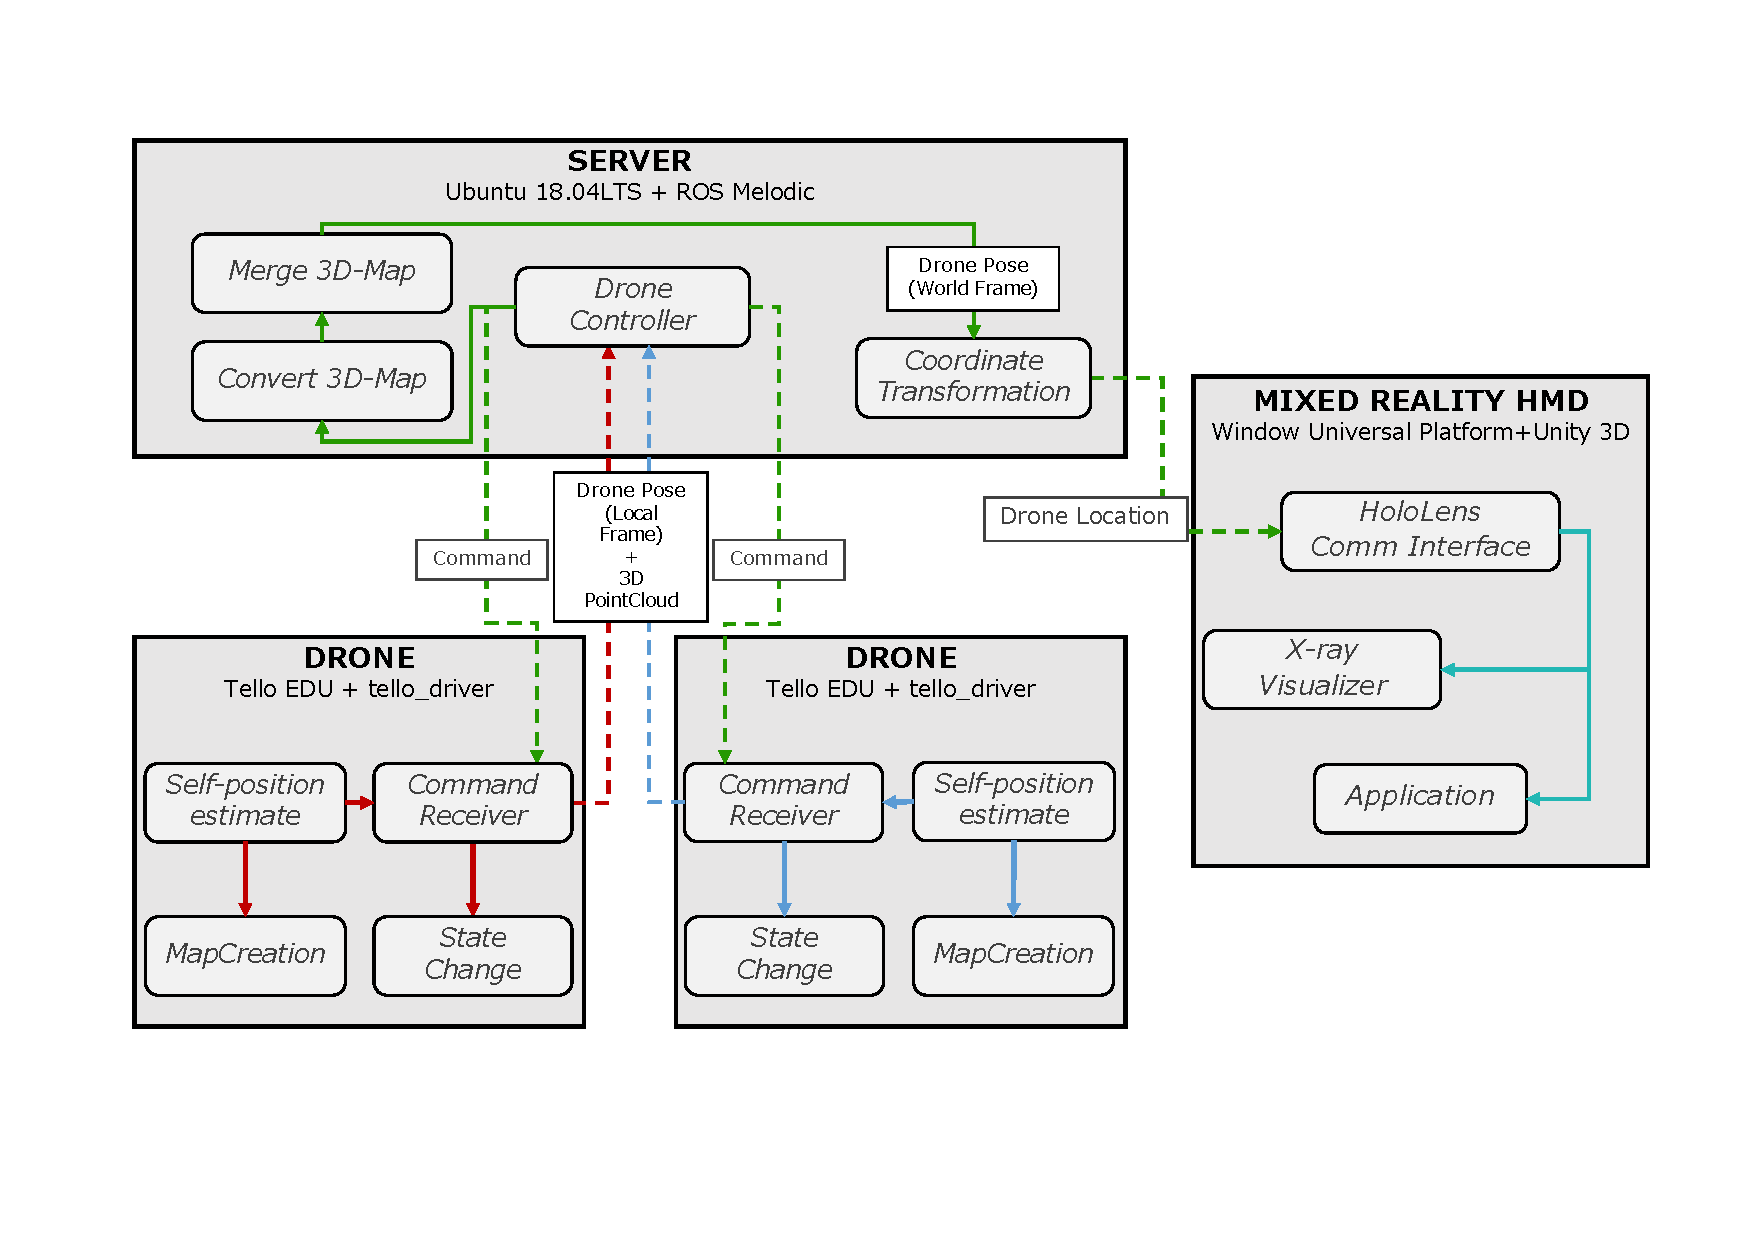
\includegraphics[width=\linewidth]{img/system.pdf}
  \caption{システム構成}
  \label{fig:system}
\end{figure}
  
% --------------------------- Section3  ---------------------------

\section{評価}

\subsection{実験と評価項目}
システム構成を図\ref{fig:system}に示す.
本研究では2つのドローン操縦方式を用意し,二人称視点方式,可視化方式と定義する.
ドローンが撮影する映像を頼りに操縦を行う従来のドローン操縦手法である二人称視点方式と,ARを用いて死角領域内の空間認識を提供した上,ドローン上部にドローンカメラ映像を映し出すことにより,一人称視点でのドローン操縦を可能とした可視化方式を提案方式と比較する.

実験環境には,赤色と緑色の異なる背景色で表示されたモニター2台を設置しており,実験参加者は,スタート地点よりドローンを移動させ,2台のモニターに表示されたランダムなテキストを,赤色のモニター,緑色のモニターの順で報告し,ドローンを着陸させるタスクを行なった.

評価項目は操縦者がタスクを完了するまでの操縦時間,障害物への衝突警告回数とする.
本研究では,実際にドローンが障害物に衝突しないように,障害物へ衝突する直前に衝突警告を表示しており,衝突警告の回数を衝突警告回数としている.

\subsection{結果と考察}
タスク完了までの平均操縦時間の評価結果を\figref{fig:05_time}に示す.
平均操縦時間,平均衝突警告回数では,rANOVAの結果,3方式の少なくともどれか一つに有意な差があった($p < 0.001 $).
Bonferroni法の多重比較($p < 0.05$)では,提案方式は二人称視点方式,可視化方式より,平均操縦時間は有意に減少することがわかった($p < 0.05$).
% しかし,可視化方式は二人称視点方式と比較して,平均操縦時間が有意に減少しなかった($p = 0.201$).
提案方式では実験環境に飛行しているもう一台のドローンのセンサ情報を統合しているため,もう一台のドローンのカメラ映像も使用しマッピングしており,
ドローン周辺を見渡す機会が少なく,操縦時間を有意に減少させていたと考察できる.

次に,障害物への平均衝突警告回数の結果を\figref{fig:05_collision}に示す.
Bonferroni法の多重比較($p < 0.05$)では,提案方式は二人称視点方式より,平均衝突警告回数は有意に減少したが($p < 0.05$),可視化方式より有意に減少しなかった($p = 0.6169$).
可視化方式はドローン周辺の三次元環境地図を復元することには時間がかかるが,カメラ映像があるため,安心してドローン操縦を行えていると推測できる.
そのため,ARにより遮蔽物の危険度を提供するだけでは不十分であり,現実環境の映像を加えることにより,操縦者の安全性をより向上させることができることを確認した.
% しかし,可視化方式は二人称視点方式と比較して,平均衝突警告回数が有意に減少しなかった($p = 0.3607$).
% また,提案方式は可視化方式と比較して,平均衝突警告回数が有意に減少しなかった($p = 0.6169$).

\begin{figure}[!tb]
  \centering
  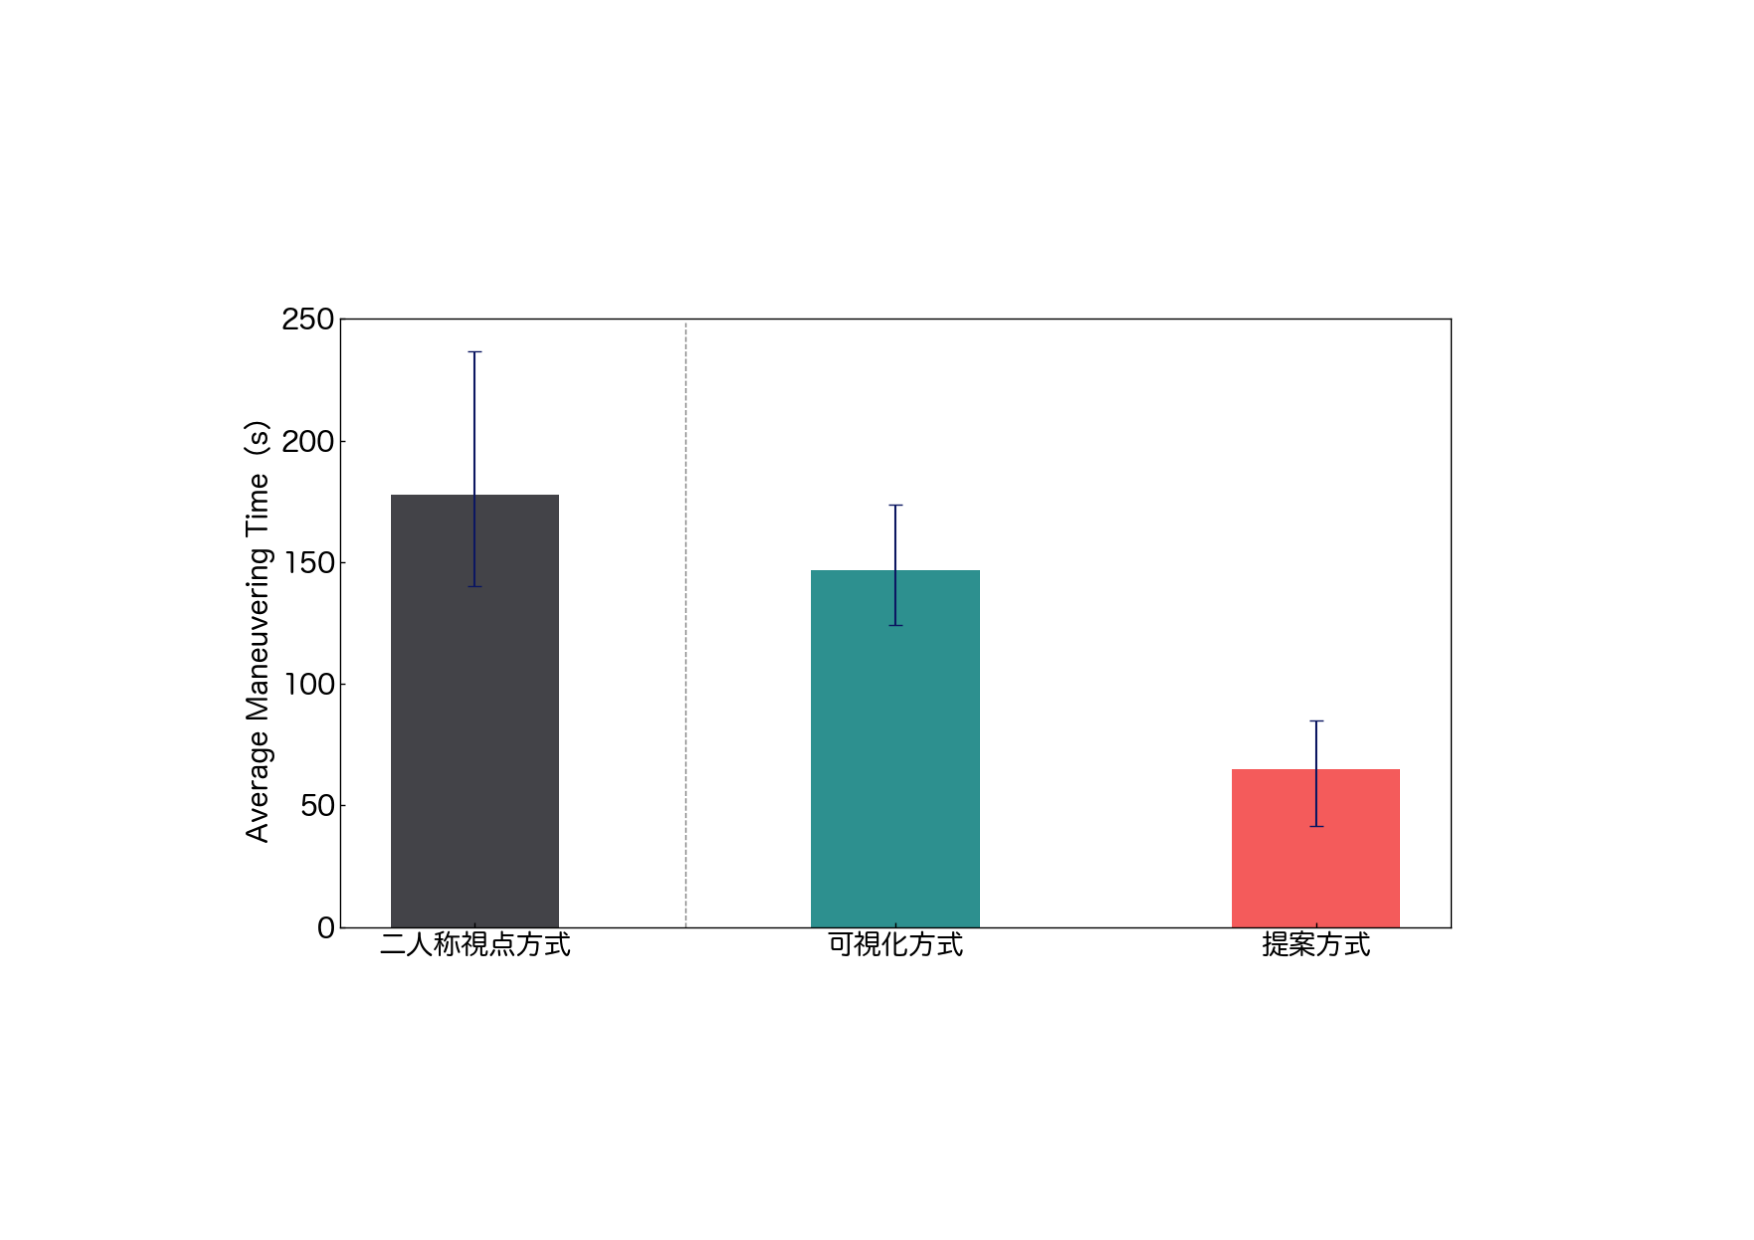
\includegraphics[width=0.9\linewidth]{img/05_time.pdf}
  \caption{平均操縦時間}
  \label{fig:05_time}
\end{figure}

\begin{figure}[!tb]
  \centering
  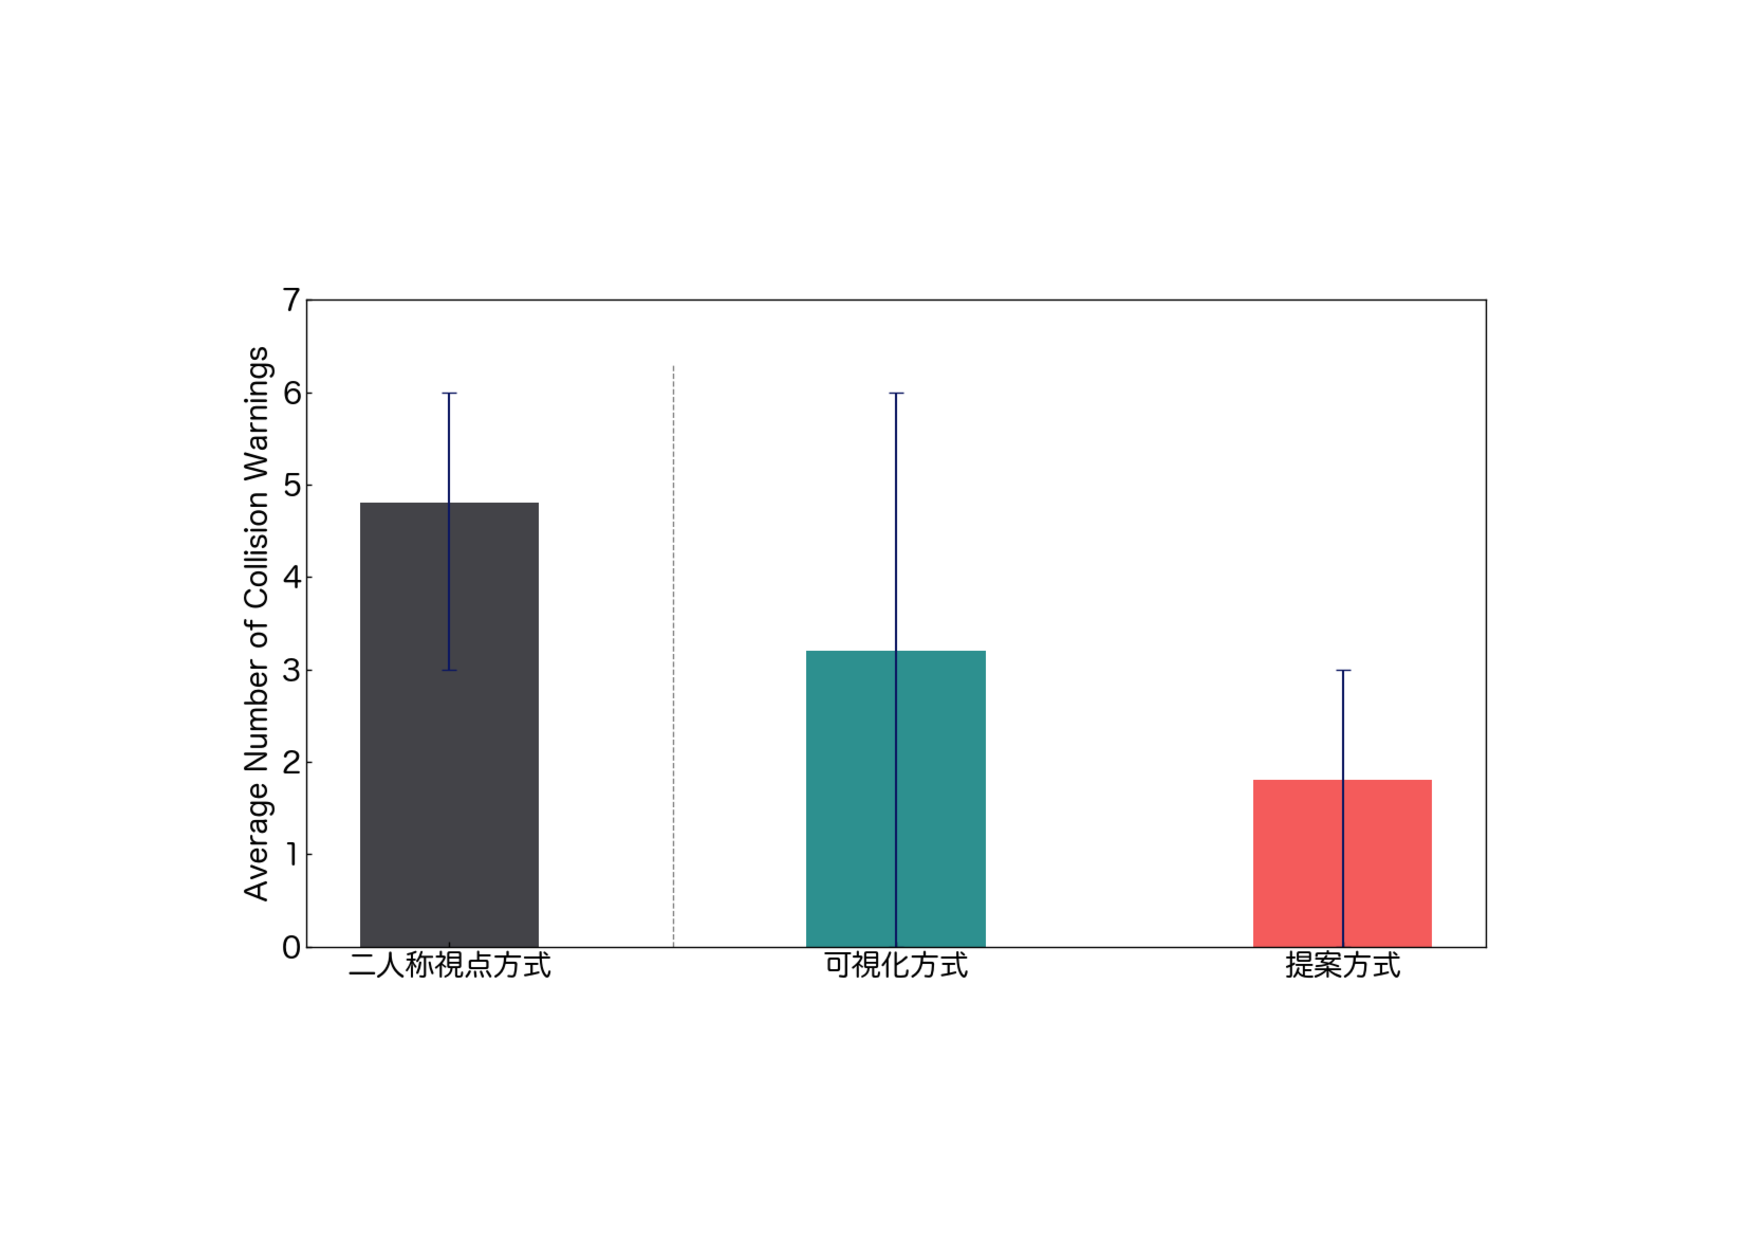
\includegraphics[width=0.9\linewidth]{img/05_collision.pdf}
  \caption{平均衝突警告回数}
  \label{fig:05_collision}
\end{figure}


% --------------------------- Section4  ---------------------------

\section{おわりに}

狭小空間の未知領域探査では,複数台のドローンを使用することで,各ドローンの走行時間を減少させ,探査効率を向上させることを期待されている.
しかし,ドローンの数が多いほど衝突のリスクは高く,また,探査領域の重複による探査効率の低下を招く可能性がある.

そこで本研究では,各ドローンがリアルタイムで取得する位置情報,三次元環境地図のセンサ情報を統合し,ARを用いて操縦者の死角領域内に存在するドローンと周辺環境を可視化する方式を提案する.
提案方式では実験環境での平均操縦時間が短く,衝突警告回数も従来の操縦手法より減少したため,未知領域探査での探査効率・安全性を向上させることを確認した.

%---------------------------------------------------------------------
% Bibliography(参考文献)
%---------------------------------------------------------------------
% thebibliography を利用する場合は以下を使用
\footnotesize{
  \begin{thebibliography}{99}
    \bibitem{Nonami}
    野波健蔵:ドローン技術の現状と課題およびビジネス最前,情報管理,Vol.59,No.11,pp.755-763(2017).
    
    \bibitem{syohou}
    山越靖之,木田哲夫,湯浅弘章:屋内空間におけるドローンの活用に関する検証 (平成 30 年度消防技術安全所の検証成果等) – (消防活動・隊員の安全管理に関する技術改良・検証),消防技術安全所報, No. 56, pp. 26–37 (2019).
    
    \bibitem{Erat}
    Erat, O., Isop, W. A., Kalkofen, D. and Schmalstieg,D.: Application of UAV imaging platform for vegeta-tion analysis based on spectral-spatial methods, {\it IEEE Transactions on Visualization and Computer Graphics}, Vol. 24, No. 4, pp. 1437-1446 (2018).
    
    \bibitem{Gupta}
    Gupta, L., Jain, R. and Vaszkun, G.: Survey of Im-portant Issues in UAV Communication Networks, IEEE Communications Surveys \& Tutorials, Vol. 18, No. 2,pp. 1123-1152 (2016).
    
  \end{thebibliography}
}

%---------------------------------------------------------------------
\end{document}
%---------------------------------------------------------------------
